%% file: example.tex = example for article-like report including BibTex 
%% init: sometime 1993 for my practical "Stellar Spectra A"
%% last: Feb  8 2015  Rob Rutten  Deil
%% site: http://www.staff.science.uu.nl/~rutte101/rrweb/rjr-edu/manuals/student-report/

%% Use the similar but empty file template.tex for writing your report

%% First read ``latex-bibtex-simple-manual'' at
%% http://www.staff.science.uu.nl/~rutte101/Report_recipe.html

%% Then run this file to see what it does:
%%    latex example     bibtex example     latex example     latex example
%% inspect with xdvi example &, or produce example.pdf for inspection.

%%%%%%%%%%%%%%%%%%%%%%%%%%%%%%%%%%%%%%%%%%%%%%%%%%%%%%%%%%%%%%%%%%%%%%%%%%%%
\documentclass{aa}    %% Astronomy & Astrophysics style class aa.cls v8.2

\usepackage{graphicx,url,twoopt,natbib}
\usepackage[varg]{txfonts}           %% A&A font choice
\usepackage{hyperref}                %% for pdflatex
%%\usepackage[breaklinks]{hyperref}  %% for latex+dvips
%%\usepackage{breakurl}              %% for latex+dvips
\usepackage{pdfcomment,acronym}      %% for popup acronym meanings
\hypersetup{
  colorlinks=true,   %% links colored instead of frames
  urlcolor=blue,     %% external hyperlinks
  linkcolor=red,     %% internal latex links (eg Fig)
}

\bibpunct{(}{)}{;}{a}{}{,}    %% natbib cite format used by A&A and ApJ

\pagestyle{plain}     %% undo the fancy A&A pagestyle 

%% Add commands to add a note or link to a reference
\makeatletter
\newcommand{\bibnote}[2]{\@namedef{#1note}{#2}}
\newcommand{\biblink}[2]{\@namedef{#1link}{#2}}
\makeatother

%% Commands to make citations ADS clickers and to add such also to refs
%% May 2014: they give error stops ("Illegal parameter number ..."}
%%   for plain latex with TeX Live 2013; the ad-hoc fixes added below let
%%   latex continue instead of stop within these commands.
%%   Please let me know if you know a better fix!
%%   No such problem when using pdflatex.
\makeatletter
 \newcommandtwoopt{\citeads}[3][][]{%
   \nonstopmode%              %% fix to not stop at error message in latex
   \href{http://adsabs.harvard.edu/abs/#3}%
        {\def\hyper@linkstart##1##2{}%
         \let\hyper@linkend\@empty\citealp[#1][#2]{#3}}%   %% Rutten, 2000
   \biblink{#3}{\href{http://adsabs.harvard.edu/abs/#3}{ADS}}%
   \errorstopmode}            %% fix to resume stopping at error messages 
 \newcommandtwoopt{\citepads}[3][][]{%
   \nonstopmode%              %% fix to not stop at error message in latex
   \href{http://adsabs.harvard.edu/abs/#3}%
        {\def\hyper@linkstart##1##2{}%
         \let\hyper@linkend\@empty\citep[#1][#2]{#3}}%     %% (Rutten 2000)
   \biblink{#3}{\href{http://adsabs.harvard.edu/abs/#3}{ADS}}%
   \errorstopmode}            %% fix to resume stopping at error messages
 \newcommandtwoopt{\citetads}[3][][]{%
   \nonstopmode%              %% fix to not stop at error message in latex
   \href{http://adsabs.harvard.edu/abs/#3}%
        {\def\hyper@linkstart##1##2{}%
         \let\hyper@linkend\@empty\citet[#1][#2]{#3}}%     %% Rutten (2000)
   \biblink{#3}{\href{http://adsabs.harvard.edu/abs/#3}{ADS}}%
   \errorstopmode}            %% fix to resume stopping at error messages 
 \newcommandtwoopt{\citeyearads}[3][][]{%
   \nonstopmode%              %% fix to not stop at error message in latex
   \href{http://adsabs.harvard.edu/abs/#3}%
        {\def\hyper@linkstart##1##2{}%
         \let\hyper@linkend\@empty\citeyear[#1][#2]{#3}}%  %% 2000
   \biblink{#3}{\href{http://adsabs.harvard.edu/abs/#3}{ADS}}%
   \errorstopmode}            %% fix to resume stopping at error messages 
\makeatother

%% Acronyms
\newacro{ADS}{Astrophysics Data System}
\newacro{NLTE}{non-local thermodynamic equilibrium}
\newacro{NASA}{National Aeronautics and Space Administration}

%% Add popups to show meaning of acronyms 
\def\acp#1{\pdftooltip{\acs{#1}}{\acl{#1}}}

%% Spectral species
\def\MgI{\ion{Mg}{I}}          %% A&A; for aastex use \def\MgI{\ion{Mg}{1}} 
\def\MgII{\ion{Mg}{II}}        %% A&A; for aastex use \def\MgII{\ion{Mg}{2}} 

%% Hyphenation
\hyphenation{Schrij-ver}       %% Dutch ij is a single character


%%%%%%%%%%%%%%%%%%%%%%%%%%%%%%%%%%%%%%%%%%%%%%%%%%%%%%%%%%%%%%%%%%%%%%%%%%%%
\begin{document}  

%% Simple header because using the A&A commands produces the A&A banner.

\twocolumn[{%
\vspace*{4ex}
\begin{center}
  {\Large \bf RYDBERG EMISSION LINES IN THE SOLAR SPECTRUM}\\[4ex] 
  {\large \bf R. J. Rutten$^{1, 2}$, M. Carlsson$^2$
              and N. G. Shchukina$^3$}\\[4ex]
  \begin{minipage}[t]{16cm} 
        $^1$ Lingezicht Astrophysics,
             NL--4158~CA Deil, The Netherlands\\
        $^2$ Institute of Theoretical Astrophysics,
             P.O.~Box 1029, Blindern, N--0315 Oslo, Norway\\
        $^3$ Main Astronomical Observatory, 
             252127 Kiev, Ukraine\\

  {\bf Abstract.~}  This is a latex and bibtex example for astronomy students,
  accompanying the manual at
  \href{http://www.staff.science.uu.nl/~rutte101/Report_recipe.html}
       {\url{http://www.staff.science.uu.nl/~rutte101/Report_recipe.html}}.
    %% this URL needs package breakurl for proper breaking when using dvips
    Note that sloppy authors wrongly use "....."
    instead of ``.....'', do not add space-making backslashes after et
    al., $\backslash$AA, etc., do not use tildes for non-breakable
    spaces before units and after initials, do not end italics with
    $\backslash${/}, do not set units in roman font, do not set the e
    of electron in roman, do not use bibtex, do not use a spell
    checker, do not use the url command for websites, do not
    link citations to \acp{NASA}'s \acp{ADS}, and probably do
    not do much else well.
    \vspace*{2ex}
  \end{minipage}
\end{center}
}] 


%%%%%%%%%%%%%%%%%%%%%%%%%%%%%%%%%%%%%%%%%%%%%%%%%%%%%%%%%%%%%%%%%%%%%%%%%%%%
\section{Introduction}     \label{sec:introduction}
%%%%%%%%%%%%%%%%%%%%%%%%%%%%%%%%%%%%%%%%%%%%%%%%%%%%%%%%%%%%%%%%%%%%%%%%%%%%
The existence of two emission features in the solar spectrum near
12~$\mu$m was announced by
\citetads{1981ApJ...247L..97M}, %% Murcray+others MgI features,
%% adding a brief comment as identifier helps to remember what paper this is
but only when they were informed by L. Testerman and J. Brault that
they had noticed them too.
Before that, \citetads{1980STIN...8031298G} %% Goldman+others IR atlas
had white-pasted them out of their spectrum atlas in the mistaken
belief that all solar and telluric lines should be in absorption.
We explained these emission features many years ago
(\citeads{1992A&A...253..567C}, % Carlsson+Rutten+Shchukina MgI
henceforth Paper~I; see also
\citeads{1994IAUS..154..309R})\footnote{%
Clicking on citations should open the corresponding \acp{ADS} abstract
page in a web browser but you may have to permit web access, for
example for Adobe Reader with the Trust Manager under Preferences. 
Likewise, hovering over an acronym should pop-up its meaning in Adobe
Reader but not with some other pdf viewers.}.

%% Add (Paper I) to the reference
\bibnote{1992A&A...253..567C}{(Paper~I)}

%% Define \PaperI as an ADS clicker
\def\PaperI{\href{http://adsabs.harvard.edu/abs/1992A&A...253..567C}{Paper~I}}

%% Note: citations are properly broken by the breaklinks hyperref option
%%   when using dvips, but then do not link in Adobe (Acrobat) Reader.
%%   Citation breaks are handled correctly by pdflatex.


%%%%%%%%%%%%%%%%%%%%%%%%%%%%%%%%%%%%%%%%%%%%%%%%%%%%%%%%%%%%%%%%%%%%%%%%%%%%
\section{Model computations}    \label{sec:computations}
%%%%%%%%%%%%%%%%%%%%%%%%%%%%%%%%%%%%%%%%%%%%%%%%%%%%%%%%%%%%%%%%%%%%%%%%%%%

\subsection{Background}
%%%%%%%%%%%%%%%%%%%%%%%%%
In the solar photosphere \acp{NLTE} departure diffusion
occurs in the upper reaches of the \MgI\ term structure (see
\PaperI\ for detail).
It is akin to optically-thin collisional-radiative recombination along
Rydberg levels in tenuous plasmas
(Fig.\,\ref{fig:waterfalls})\footnote{%
  Figure production: I usually prepare separate figures, each with
  full axis annotation, and paste these together into multi-panel
  layout using the latex commands in
  \href{http://www.staff.science.uu.nl/~rutte101/rrweb/rjr-edu/manuals/student-report/cutmultipanel.tex}{\url{cutmultipanel.tex}}.
  They remove superfluous axis annotation between adjacent panels and
  rescale them to the same size.
  This way I choose the assembly layout while writing the paper.}.

%% {fig:waterfalls}
%===========================================================================
\begin{figure}[hbtp]
  \centering
  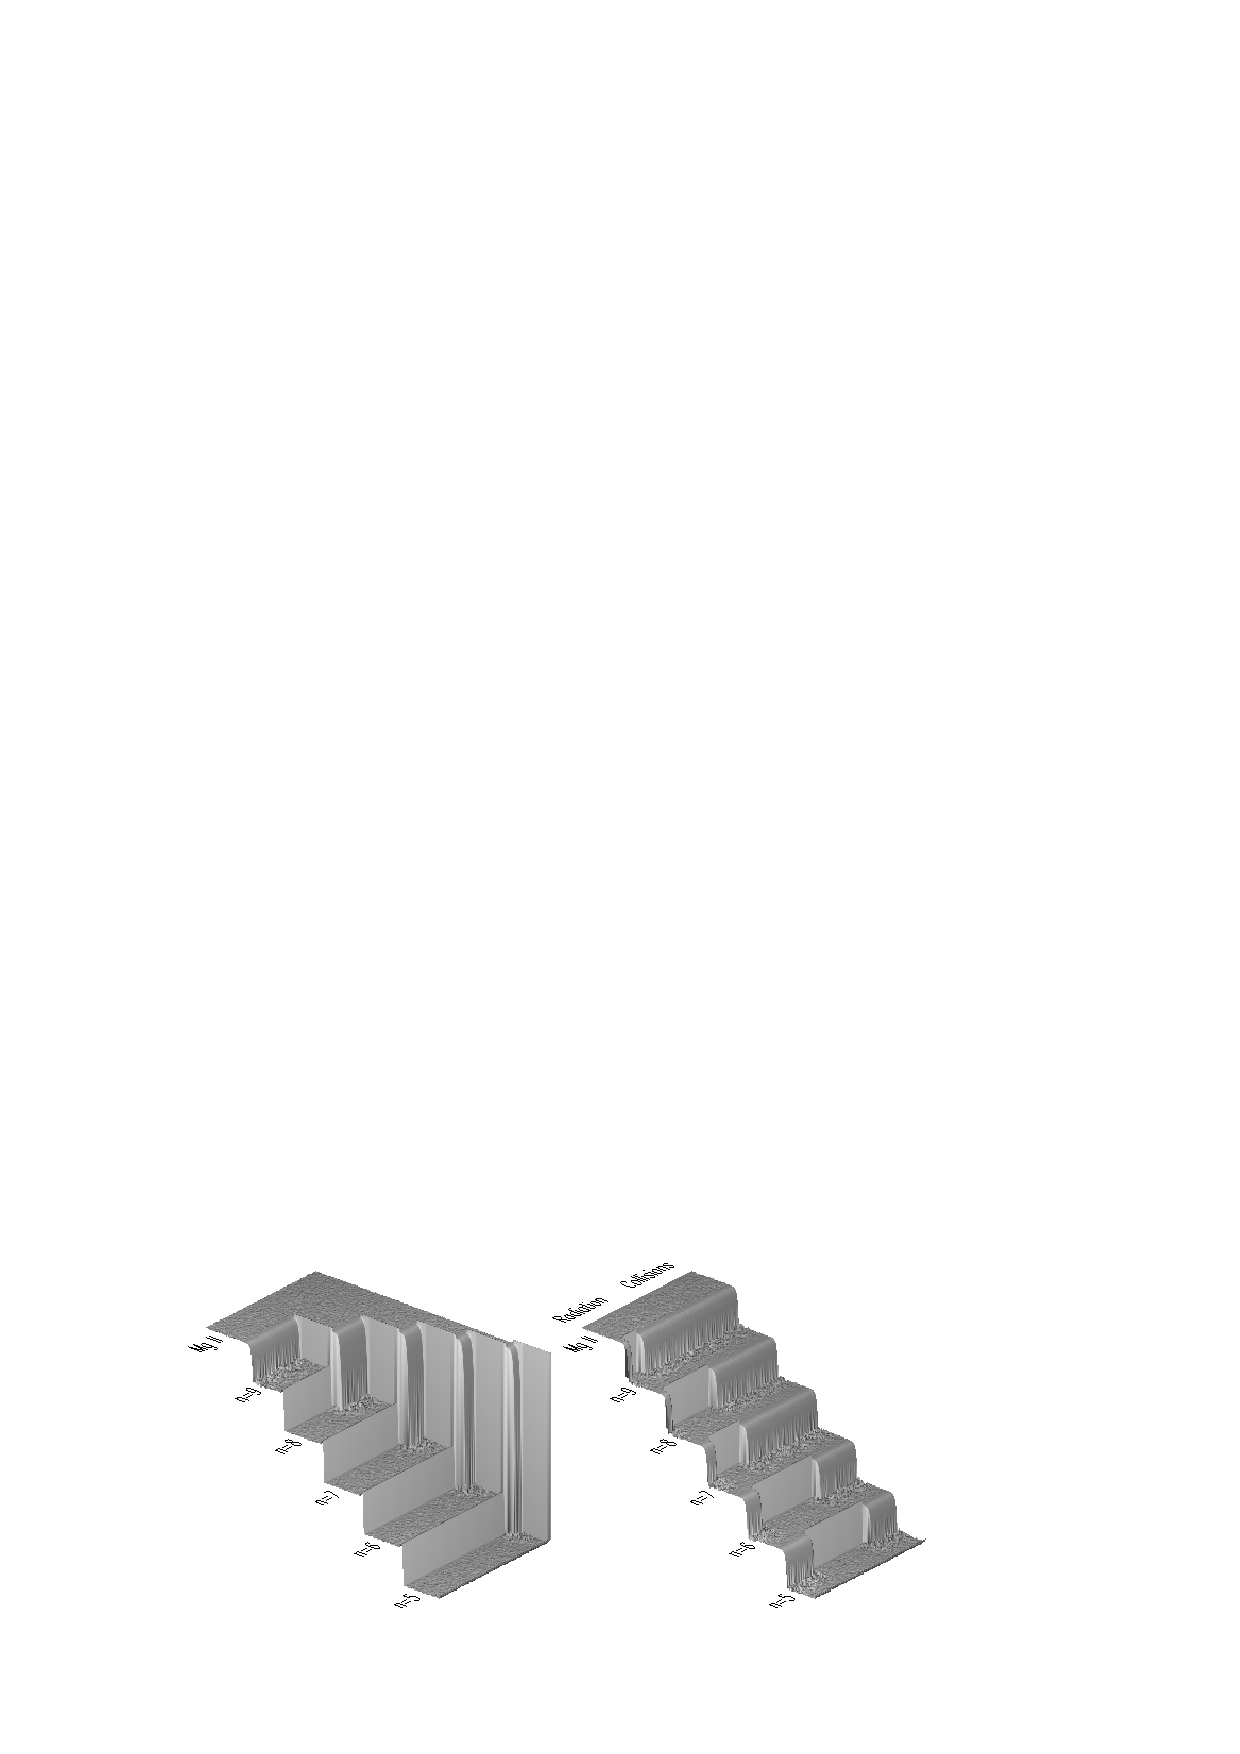
\includegraphics[width=\columnwidth]{waterfalls}  %% file name without extension
  \caption[]{\label{fig:waterfalls} %
    Collisional-radiative recombination along \MgI\ Rydberg states
    visualized for pool-drop kayakers.
    The lefthand sketch shows that the largest recombination flow from
    the magnesium population reservoir in the \MgII\ ground state is
    into the highest \MgI\ level ($n\!=\!9$ in our model).
%% the ! signs above reduce the spacing around the =    
    The righthand sketch shows that along the $\Delta n\!=\!1$
    downward ladder the flow is initially dominated by collisional
    transitions but that radiative transitions take over.
    The flow is driven by photon losses in strong \MgI\ lines and is
    balanced by radiative ionization in ultraviolet edges.
    Similar Rydberg flows occur in other elements, but the \MgI\
    Rydberg levels have the largest photospheric populations, even
    exceeding the hydrogen ones.
    From
    \citetads{1994IAUS..154..309R}. % Rutten+Carlsson Tucson review
  }
\end{figure}
% ===========================================================================
%% always have "floats" such as figures between blank lines

%% Note that in this file every sentence starts on a new line,
%% for better readability, easier change, and better synchronization
%% in shared-access systems such as svn.
%% This is automatically formatted by emacs in the setup I use,
%% specified in my ~/.emacs (shown in "Recipes for linux/unix/MacOSX"
%% on my website).


\subsection{Method}
%%%%%%%%%%%%%%%%%%%%
We solved the statistical equilibrium and radiative transfer equations
for all relevant levels and frequencies in \MgI\ and \MgII\ for
various models of the solar atmosphere, including the standard one
formulated in the monumental papers by Vernazza et al.\
(\citeyearads{1973ApJ...184..605V}, % VALI
\citeyearads{1976ApJS...30....1V}, % VALII
\citeyearads{1981ApJS...45..635V}). % VALIII
%% example same-author citation list


%%%%%%%%%%%%%%%%%%%%%%%%%%%%%%%%%%%%%%%%%%%%%%%%%%%%%%%%%%%%%%%%%%%%%%%%%%%%
\section{Conclusion} \label{sec:conclusion}
%%%%%%%%%%%%%%%%%%%%%%%%%%%%%%%%%%%%%%%%%%%%%%%%%%%%%%%%%%%%%%%%%%%%%%%%%%%%
Our computation explained the formation of the enigmatic
\MgI\,12\,$\mu$m emission features.
They arise through population depletion by line photon losses and
population replenishment from the ionic reservoir through highly
excited levels.
A Rydberg-channel replenishment flow is realized by
collisionally-dominated population diffusion via ladder-wise departure
divergence (see Fig.~\ref{fig:waterfalls} in
Sect.~\ref{sec:computations}).  
%% note the tilde.  Fig. \ref would generate too much end-of-sentence space
%% and a line break between Fig. and the number is undesirable

%%%%%%%%%%%%%%%%%%%%%%%%%%%%%%%%%%%%%%%%%%%%%%%%%%%%%%%%%%%%%%%%%%%%%%%%%%%%
\begin{acknowledgements} %% acronym popups do not work in here, why?
We are indebted to \acp{NASA}'s \href{http://adsabs.harvard.edu}{ADS}
for its magnificent literature and bibliography serving (used here,
but unknowingly missed in pre-internet 1992).
\end{acknowledgements}

%%%%%%%%%%%%%%%%%%%%%%%%%%%%%%%%%%%%%%%%%%%%%%%%%%%%%%%%%%%%%%%%%%%%%%%%%%%%
%% references
\bibliographystyle{aa-note} %% aa.bst but adding links and notes to references
%%\raggedright              %% only for adsaa with dvips, not for pdflatex
\bibliography{example}    %% example.bib = bibtex entries copied from ADS

\end{document}

